\chapter{Existující nástroje}

V této kapitole zanalyzujeme některé existující nástroje pro kresbu diagramů.
Nástroje lze rozdělit do tří skupin -- návrh diagramů konceptuální vrstvy,
logické vrstvy a nástroje pro kresbu libovolných diagramů.

\section{ERDPlus}

ERDPlus je modelovací nástroj pro tvorbu ER diagramů, relačních schémat a
hvězdicových schémat. Aplikace je dostupná ve webovém prohlížeči na adrese
\url{erdplus.com}. Její uživatelské rozhraní je tedy vyvinuto ve standardních
webových technologiích -- HTML, CSS a JavaScript -- a dále využívá framework
React pro tvorbu rozhraní v jazyce JavaScript.

ERDPlus lze používat bez založení uživatelského účtu a vytvořený diagram
exportovat do speciálního formátu erdplus, nicméně uživatel tak přijde o možnost
využití úložiště diagramů na serveru aplikace. Služby ERDPlus nejsou žádným
způsobem zpoplatněny.

Tvorba ER diagramů je intuitivní s jednoduchým uživatelským rozhraním, které je
vidět na obrázku \ref{fig:erdplus}. Uživatel má na výběr mezi vytvořením entity,
atributu, relace, spojení mezi těmito objekty a jednoduchého textového popisku.
V pravé části rozhraní se nachází panel s vlastnostmi zvoleného objektu. V tomto
panelu může uživatel také rychleji tvořit atributy entit a relací. Při zvolení
relace lze v panelu zvolit entity, které mají být v relaci, a spojení je pak
automaticky vytvořeno. Zároveň lze zvolit jednotlivé multiplicity relace.

ER diagram lze exportovat do rastrového formátu PNG. Zajímavou funkcí je také
převod do relačního schématu. Tato funkce je dostupná pouze tehdy, když uživatel
ER diagram uloží na server ERDPlus. Poté zvolí možnost \emph{Convert to
Relational Schema} a ERDPlus vytvoří nové relační schéma. Z relačních schémat
lze podobně vygenerovat SQL.

\begin{figure}
  \centering
  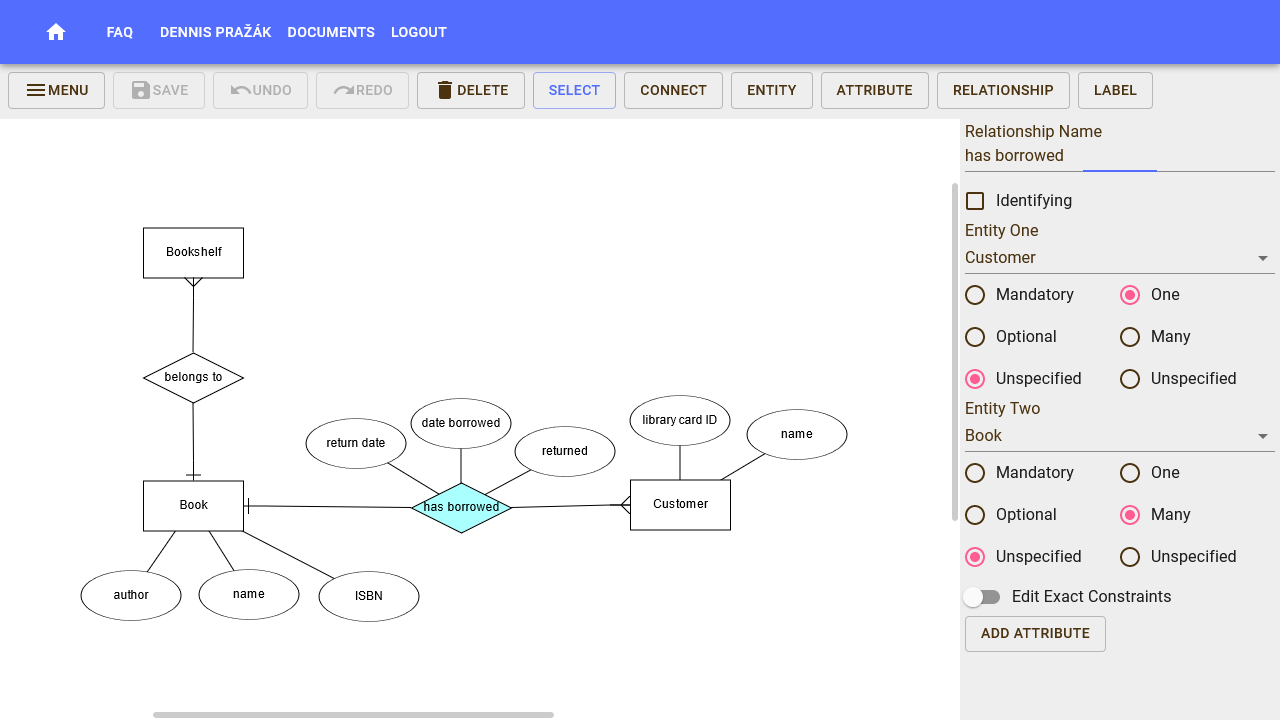
\includegraphics[width=\textwidth]{../img/erdplus.png}
  \caption{Tvorba ER diagramu v ERDplus}
  \label{fig:erdplus}
\end{figure}

\section{drawSQL}

drawSQL je modelovací nástroj pro tvorbu relačních schémat. Aplikace je dostupná
ve webovém prohlížeči na adrese \url{drawsql.app}. Je vyvinuta ve standardních
webových technologiích a používá framework Vue.js. Plán zdarma umožňuje tvorbu
veřejně přístupných diagramů, které mohou mít maximálně 15 tabulek (entit).
Měsíčně placené plány umožňují vytvářet neveřejné diagramy, více (až nekonečně
mnoho) tabulek v diagramu, více uživatelů, kteří mohou na diagramu spolupracovat
a přístup k verzovacím nástrojům.

Hlavní funkcí drawSQL je export schématu do SQL. Proto si uživatel při vytváření
diagramu zvolí cílovou databázi, pro kterou schéma tvoří. Výsledné SQL tak bude
mít tvar, se kterou cílová databáze umí pracovat. Podporovanými databázemi jsou
MySQL, PostgreSQL a SQL Server.

Rozhraní, které je vidět na obrázku \ref{fig:drawsql}, obsahuje diagram a
postranní panel. V postranním panelu lze vytvářet jednotlivé tabulky, definovat
jejich sloupce a vlastnosti jednotlivých sloupců -- typ sloupce, nullability,
zda se jedná o primární klíč, unikátní klíč nebo index. Tyto změny se v reálném
čase reflektují v diagramu, ve kterém může uživatel jednotlivé sloupce spojovat,
čímž vytváří cizí klíče. Pozici těchto lomených čar lze upravovat pouze
posunutím tabulky v diagramu. Pokud je cizích klíčů víc, začne být diagram velmi
nepřehledný.

Diagram lze importovat ze souboru SQL stisknutím File $\rightarrow$ Import.
Stisknutím tlačítka File $\rightarrow$ Export se otevře nabídka Export, ve které
může uživatel diagram exportovat do SQL své předem zvolené databáze, nebo do
rastrového obrázku ve formátu PNG. Vývojáři aplikace plánují implementovat také
export diagramu pomocí serializace do formátu JSON. V nabídce Export je navíc
možnost nechat si vygenerovat platformně specifický kód jako například migrační
třídy pro Laravel, definice modelů pro Laravel a migrační schémata pro AdonisJS.

\begin{figure}
  \centering
  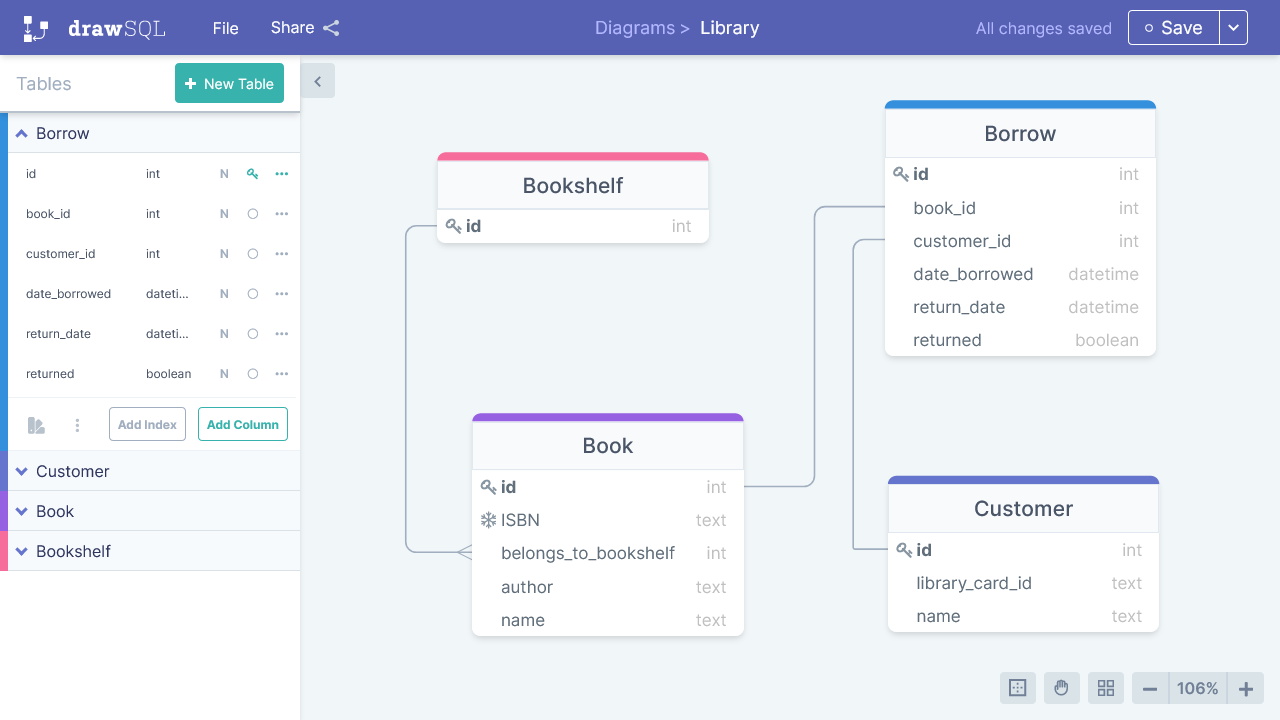
\includegraphics[width=\textwidth]{../img/drawsql.png}
  \caption{Tvorba diagramu v drawSQL}
  \label{fig:drawsql}
\end{figure}

\section{diagrams.net}

diagrams.net (dříve draw.io) je obecný open-source kreslící nástroj vydaný s
licencí Apache License 2.0, dostupný jako webová aplikace na adrese
\url{app.diagrams.net} nebo jako desktopová aplikace. Desktopová verze aplikace
je sestavena stejným způsobem jako webová, pouze je zabalena pomocí platformy
Electron do okna Chromium. Je vyvinut v běžných we\-bo\-vých tech\-no\-lo\-gi\-ích (Java\-Script,
CSS, Html).

Soubor lze uložit do serializovaného XML formátu .drawio, rastrového formátu
PNG, vektorového formátu SVG a jako dokument HTML. Jako úložiště lze využít
Google Drive, OneDrive, Dropbox, GitHub, GitLab, vlastní počítač (stažení) nebo
paměť webového prohlížeče. Ze stejných typů souborů lze diagram také importovat.
Při importu rastrového formátu však uživatel ztratí možnost diagram editovat.

Uživateli jsou v levém postranním panelu k dispozici standardní tvary ER
diagramů, UML diagramů, flowchart diagramů a další základní tvary pro kresbu
diagramů. Tvary lze libovolně kombinovat a spojovat podržením levého tlačítka a
tažením myší z a do kotev na krajích objektů. Každý objekt a spojovací čára má
vlastnosti, které lze upravovat v pravém postranním panelu. Upravovat lze jak
vlastnosti a styly formátu SVG, tak nad nimi nastavěné vlastnosti vyššího řádu,
jako například konce šipek.

Uživatelské rozhraní, které je vidět na obrázku \ref{fig:diagrams.net} je velmi
podobné kancelářským aplikacím Google. Je tak přívětivé pro nové uživatele,
kteří již s aplikacemi Google dříve pracovali.

\begin{figure}
  \centering
  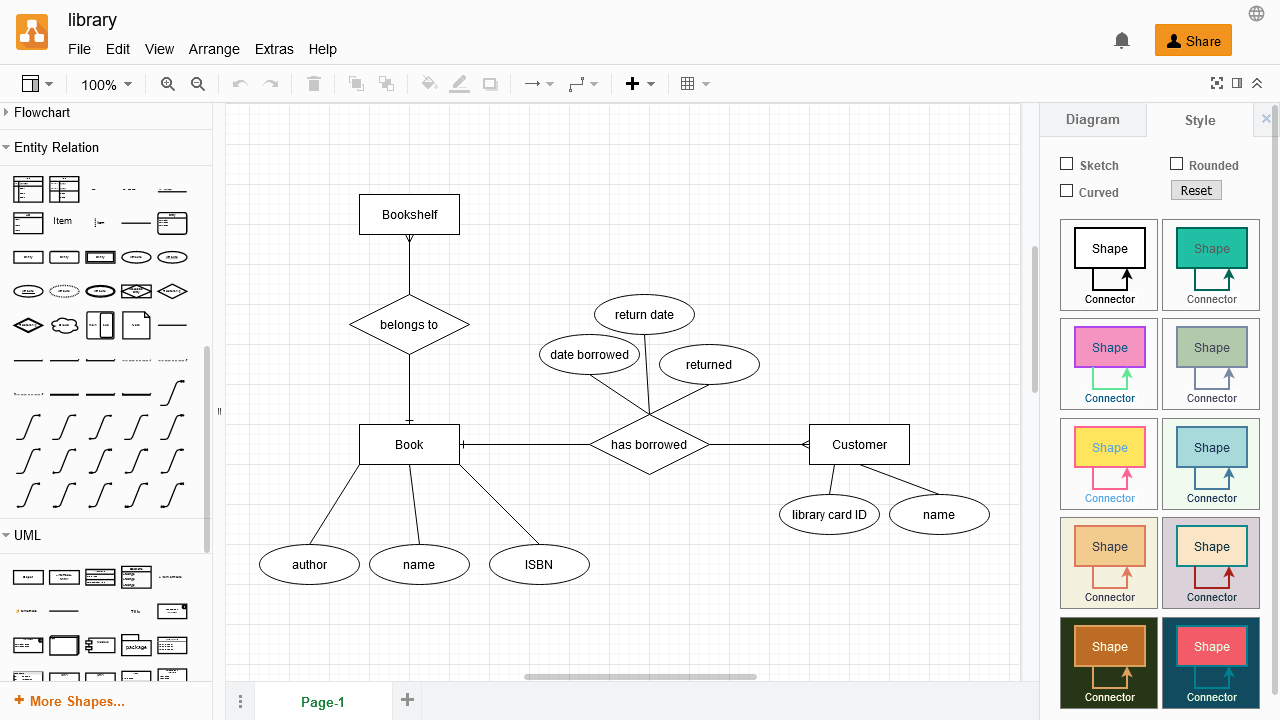
\includegraphics[width=\textwidth]{../img/diagrams.net.png}
  \caption{Tvorba ER diagramu v aplikaci diagrams.net}
  \label{fig:diagrams.net}
\end{figure}

\begin{table}
  \centering
  \begin{tabular}{c|cccc}
    aplikace      & ER          & rastrový export   & SQL export & vektorový export \\
    \hline
    ERDplus       & \checkmark  & \checkmark        & \checkmark & \\
    drawSQL       &             & \checkmark        & \checkmark & \\
    diagrams.net  &\checkmark   &\checkmark         &            &\checkmark
  \end{tabular}
  \label{tab:criteria}
  \caption{Srovnání možností exportu diagramu jednotlivých aplikací}
\end{table}


\begin{table}
  % TODO: fix

  \begin{minipage}{12cm}
    \centering
    \begin{tabular}{c|cc}
      aplikace  & online úložiště & živá spolupráce \\
      \hline
      ERDplus   & \checkmark      &\                  \\
      drawSQL   & \checkmark\footnote{zdarma pouze pro veřejné diagramy} & \checkmark\footnote{pouze v placené verzi} \\
      diagrams.net&\checkmark\footnote{využívá úložiště třetí strany} & \checkmark\footnote{využívá úložiště třetí strany}
    \end{tabular}
  \end{minipage}
  \caption{Srovnání dalších funkcí jednotlivých aplikací}
\end{table}